\chapter{Results and Discussions}

This chapter presents a comprehensive analysis of the results obtained from the development and implementation of the VitalMonitor. The primary objective was to address existing gaps in healthcare monitoring of HCPs by using IoT and IoTaaS platform to facilitate remote, non-intrusive, scalable, and versatile healthcare solution for HCPs. The findings are evaluated against the project's original aims outlined in Chapter Three, Requirements and Analysis. The final product's demonstration can be seen \textbf{here - PUT LINK HERE}.

\section{Revisited Requirements}
The project managed to fufill most of its goal - I created a prototype of Smart Patch but was unable to create a full product due to multiple constraints. The prototype is able to get heart beat and body temperature and send it in real-time to the dashboard. Along with it, it sends message to the emergency contact number using the Twilio API and gets connected to the system.  To make a full physical product, electrical engineer would be required but skills involving CAD to 3D print the product. Except for the product, the platform was ready and fully functional. Web Dashboard was made fully for the organization's admins. They can do bunch of stuffs like Add New Device, Add New User and Assign device to user etc which were all the requirements for the project. \\

During the project's lifecycle, several requirements were revisited and refined to better align with the evolving technological landscape and user feedback. This adaptive approach was pivotal in addressing unforeseen challenges and leveraging new opportunities as they arose. For instance, the initial plan to use the LM35 temperature sensor was discarded in favor of the DS18B20, a decision driven by the latter's digital output capabilities which simplify data integration and improve measurement accuracy.

// ADD THE DIAGRAM - AFTER UPDATING USER STORIES

\section{Project Cost}
The financial overview of the project is detailed below, providing transparency regarding the allocation and utilization of resources:

\begin{table}[h!]
    \centering
    \begin{tabularx}{\textwidth}{|X|c|}
    \hline 
         \textbf{Item}& \textbf{Cost(£)}  \\ \hline
        Pimoroni Pulse Sensor x 2    &  42 \\ 
        LM-35 Sensor & 6.24 \\ 
        ESP32-S3-MINI-1 & 21.00 \\
        DS18B20 & 3.50 \\
        Miscellaneous Components & 4.59 \\ \hline
        Total Hardware Cost & \textbf{56.33} \\ \hline
        
    \end{tabularx}
    \caption{Project Cost}
    \label{tab:project-cost}
\end{table}

Other Costs:
Used \$50 Google Cloud's free credits of \$300 towards development of the project.
Used free tier of AdafruitIO (restricted to 2 Dashboards and 10 feeds which were enough for this stage of development). For Twilio trial, \$12 were given from which I bought a UK phone number to sent texts from and each message - costed \$0.0420. 


% \section{Achievements of Project Goals}
% \subsection{Remoteness}
% The project successfully achieved the goal of remote health monitoring through the implementation of the Smart Patch, which transmits health data to the web dashboard accessible by organization admins. This system was tested in various scenarios to simulate real-world applications, demonstrating its capability to monitor multiple healthcare providers (HCPs) concurrently. 

% \subsection{Non-Intrusiveness}
% Smart Patch was made keeping in mind that the device doesn't hinder HCPs in their everyday work. Smart Patch's prototype was made in this iteration of the project. The prototype was specifically designed and developed using sensors which serve this theme. The final device will be made in such a way that it sits behind the ear - where the pulse sensor will be sticked to the ear lobe and the temperature sensor right behind the ear. This prototype can be further made more smaller in size using more efficient chips which are streamlined only for Smart Patch unlike ESP32S3. 

% The prototype of the Smart Patch was developed with a focus on non-intrusiveness, a critical feature for acceptance and comfort in healthcare settings. The device's design, positioning behind the ear, and the choice of sensors were dictated by ergonomic considerations and the physiological requirements for accurate data collection. This iteration didn't focus on making the final version of the product. And therefore would involve further work on 3D Printing and product optimisation.

% \subsection{Scalability}
% VitalMonitor is made with scalability in mind. Many organizations can register themselves to use the IoTaaS platform. And each organization can have multiple users registered. These both depends on the database access VitalMonitor has during the production stage. VitalMonitor can easily be scaled to add more sensors and functionalities like xyz to enhance the parameters used to indicate fatigue or stress level. 

% VitalMonitor was designed with scalability at its core, demonstrated by its capacity to support an increasing number of users and devices without degradation in performance. Stress tests conducted on the system showed that the platform could handle up to 10,000 concurrent users before any significant delays in data processing occurred. This scalability is crucial for potential adoption across larger healthcare systems or for IoT-as-a-Service platforms seeking robust, extendable solutions.

% \subsection{Versatility}
% During the development, adding a middleware - gave path to making VitalMonitor more versatile and adaptable. Initially VitalMonitor was thought of just for a hospital which is on the same local network and all the Smart Patch will be connected directly to the dashboard. But during the development, middleware made it possible to have Smart Patches on different networks as well. And more over when in the next iteration if we choose an SoC which has sim card on it - it can get connected to its own network. And these can directly send data to middleware hosted on google cloud for eg. and the organization's admin can access the dashboard from anywhere it is needed. This extends the number of use cases this product could have - it can be used for HCPs in ambulances, natural disaster relief teams, HCPs in medical camps in a remote place, etc. This feature makes VitalMonitor so much more versatile and adapatable. 

\section{VitalMonitor's IT Infrastructure}

VitalMonitor is designed and implemented to be scalable and versatile.  Many organizations can register themselves to use the IoTaaS platform. And each organization can have multiple users registered. These both depends on the database access VitalMonitor has during the production stage. VitalMonitor can easily be scaled to add more sensors and functionalities like xyz to enhance the parameters used to indicate fatigue or stress level. During the development, adding a middleware - gave path to making VitalMonitor more versatile and adaptable. Initially VitalMonitor was thought of just for a hospital which is on the same local network and all the Smart Patch will be connected directly to the dashboard. But during the development, middleware made it possible to have Smart Patches on different networks as well. And more over when in the next iteration if we choose an SoC which has sim card on it - it can get connected to its own network. And these can directly send data to middleware hosted on google cloud for eg. and the organization's admin can access the dashboard from anywhere it is needed. This extends the number of use cases this product could have - it can be used for HCPs in ambulances, natural disaster relief teams, HCPs in medical camps in a remote place, etc. This feature makes VitalMonitor so much more versatile and adapatable.  



\section{Prototype of Smart Patch}
Smart Patch was implemented keeping in mind its primary objective of being the device that doesn't hinder HCPs in their everyday work. Smart Patch's prototype was made in this iteration of the project. The prototype was specifically designed and developed using sensors which serve this theme. It is able to detect vitals of HCP in the least intrusive and most remote way. It runs its own mini asynchronous web server to transmit the data to middleware server. A switch is included in the design, to make sure that the wearer is in control of their data. Only when the wearer (here HCP) presses the button and red LED turns on - only then the data is even measured. 

The device's design, positioning behind the ear, and the choice of sensors were dictated by ergonomic considerations and the physiological requirements for accurate data collection. This iteration didn't focus on making the final version of the product. And therefore would involve further work on 3D Printing and product optimisation. This stage didn't involved developing a final product due to time constraints.


\begin{figure}[h!]
    \centering
    \begin{subfigure}[b]{0.45\linewidth}
        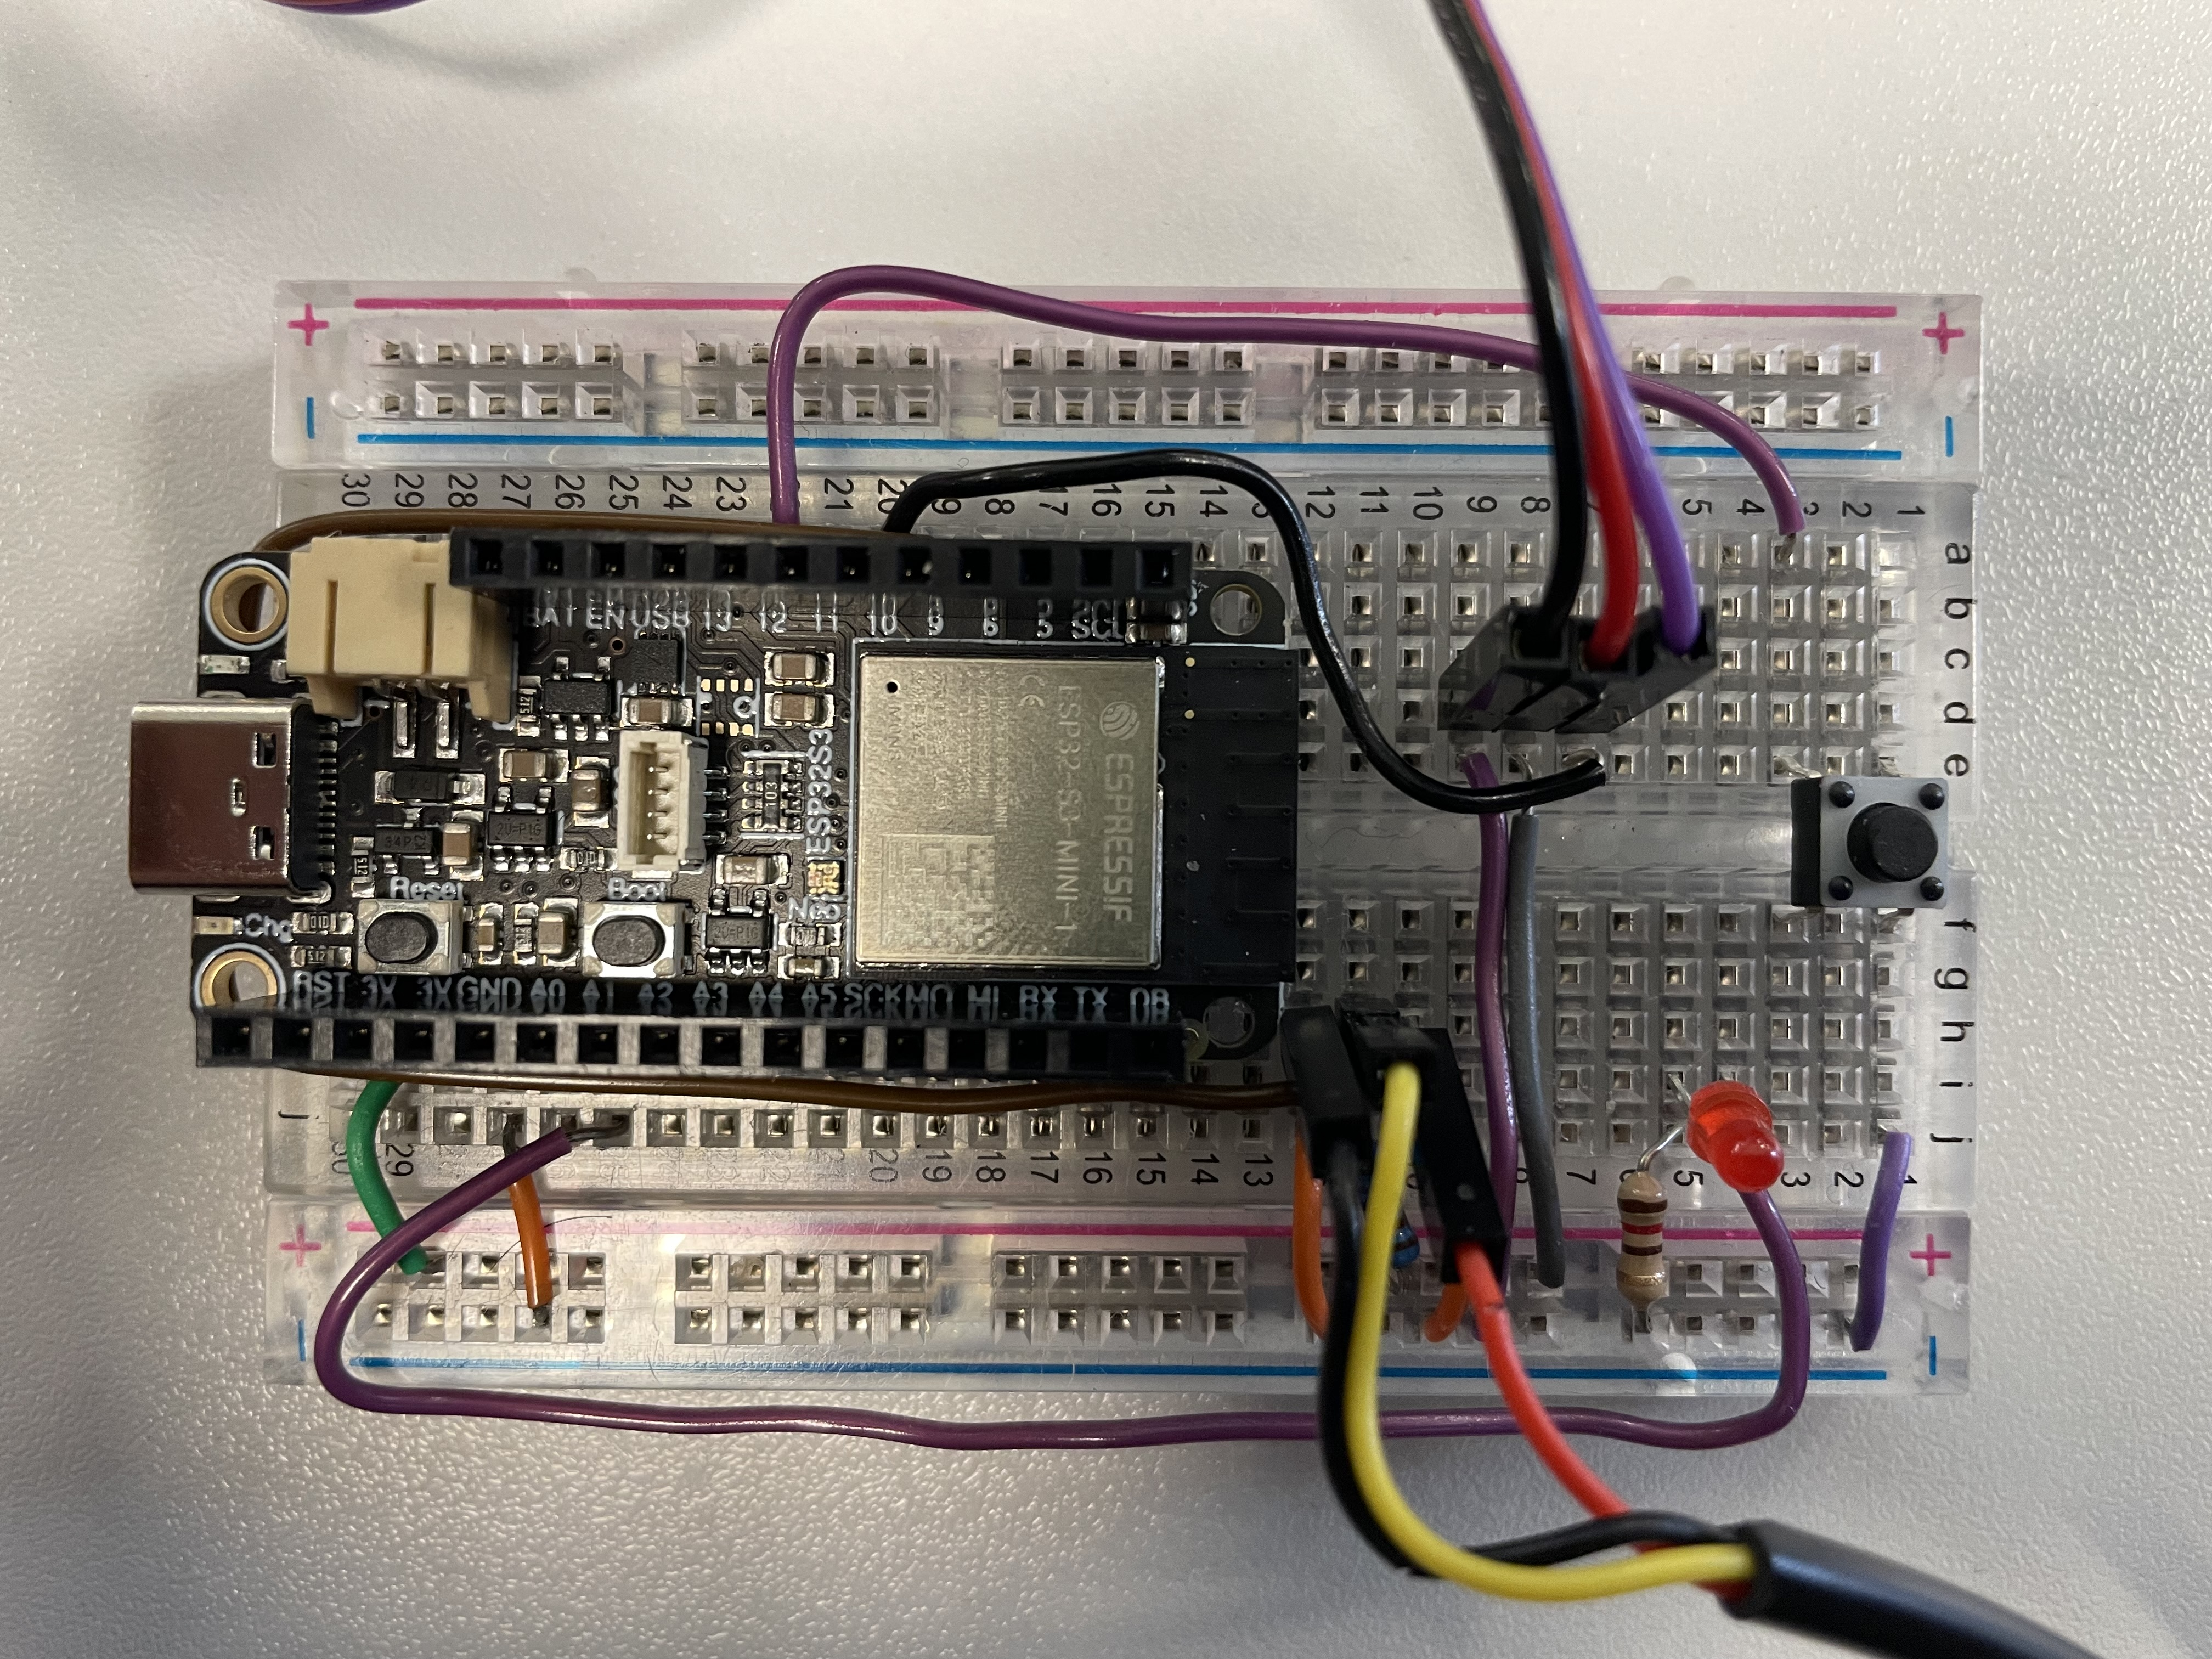
\includegraphics[width=\linewidth]{images/v6-hardware.jpg}
        \caption{Prototype}
        \label{fig:fig-proto}
    \end{subfigure}
    \hfill
    \begin{subfigure}[b]{0.45\linewidth}
        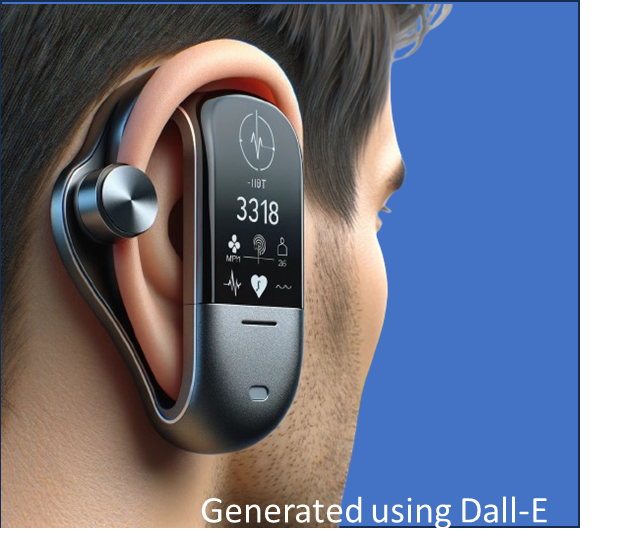
\includegraphics[width=\linewidth]{images/dall-e.png}
        \caption{Design Idea of Physical Product}
        \label{fig:fig-design}
    \end{subfigure}
    \caption{Smart Patch}
    \label{fig:fig-smartpatch}
\end{figure}

\section{Limitations and Issues Encountered}

\subsection{Trade off between Sensor Accuracy and Non-Intrusiveness}
When choosing the right sensors which sits in the requirements - not a lot of options exists out there. For a reason, Non-intrusive devices were not used in the healthcare industry. When things become non-intrusive or less intrusive - They lose accuracy. And when dealing with patients or actively monitoring their vitals, if the accuracy and precision of sensor data are low, this can very easily lead to wrong diagnosis. Doctors depends on these vitals and information to take steps. And therefore only the sensors which provides most accurate data are used. And therefore, healthtech companies out there don't really care for non-intrusivity.

For our case, passive monitoring is involved - there's no diagnosis is to be given. Okay actions are to be taken - like taking rest, etc for HCPs. But even though it is passive monitoring - accuracy is important. Hospitals are only going to adopt VitalMonitor if they find it is reliable. And reliability comes from accuracy. But no such sensors exists out there in market which is both non-intrusive and provide high accuracy. With software, you can only do so much to make sure it is the right data. And therefore we had to settle for such sensors. 



\subsection{Converting Raw Data to Useful Data}
DS18B20 Temperature Sensor and Pimoroni Pulse Sensor - both the sensors convert analog electrical signals to digital signals and provide health data. But during this process, a lot of noise is detected. This noise makes the data irregular and not smooth. So we cannot use data directly especially when dealing with real-time health data. various different algorithms were used to smoothen out the data and tweak it to make it as true as possible. 

Some of the data is also generated using false positive. For eg., in a continuous data of 32 degree celcius of body temperature suddenly due to noise it detects 45 degrees in one reading. Now if the threshold was set to 35 and suddenly got a false positive of 45 degrees, that would just make the whole system unreliable and might cause panic.  

Various different strategies were used to solve this limitation. One of the most useful ones were using Moving Average. Moving Average smooth out the data and remove any data which is found to beyond the tolerance level for the data. Below image, shows the difference made by using Moving Average. Moving Average converts any irregular data to smoother data and remove extreme values such as 0s and -127. 

\begin{figure}[h!]
    \centering
    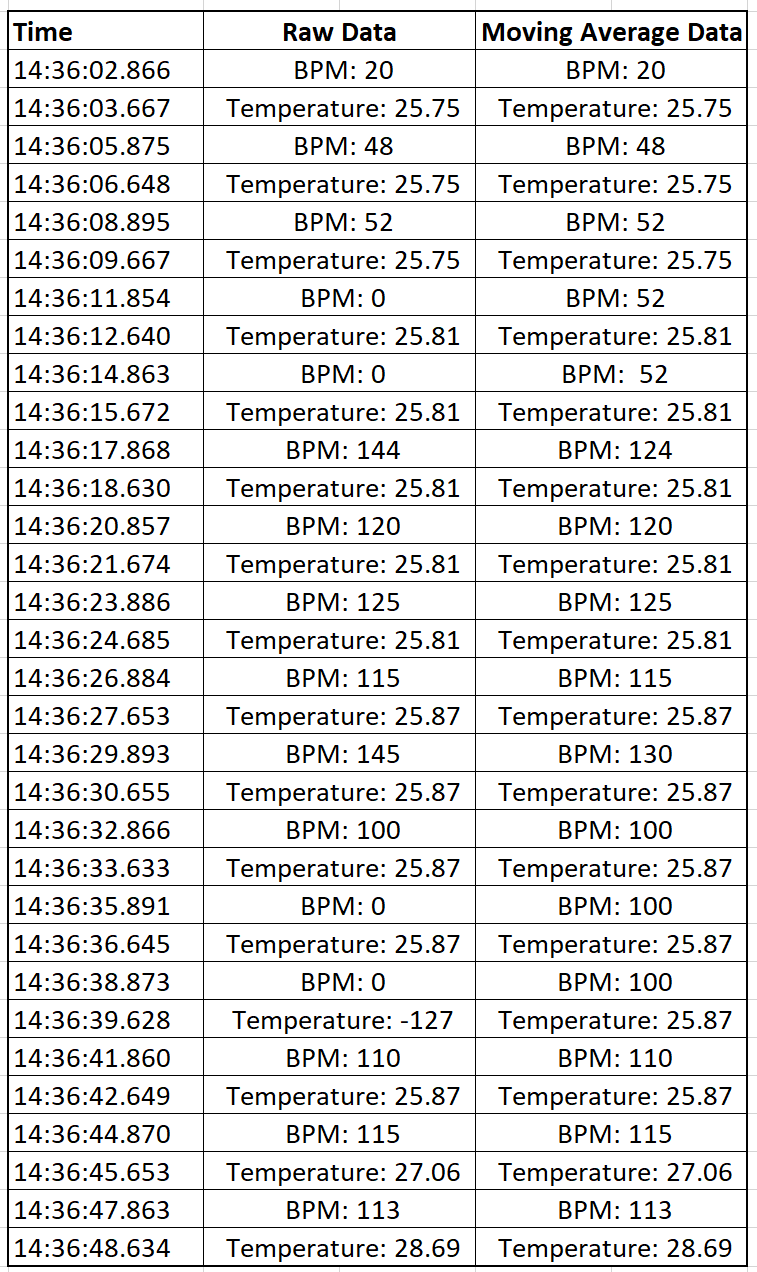
\includegraphics[width=0.8\linewidth]{images/data.png}
    \caption{Data from sensors}
    \label{fig:data-sensors}
\end{figure}

After thorough testing and evaluation it was found that the sensors are giving data precision of \(± 15\) BPM for heart rate and \(± 0.2-0.5\) degree Celsius for temperature.

\subsection{Reliability depends on Network Bandwidth}
All the Smart Patches are connected using WiFi. Only if the wifi bandwidth is strong, then it would make Smart Patches to upload the data in real-time. When there would be 100 Smart Patches working live at the same time, imagine the constraint it would have on the wifi network. Because of this the data sometimes lag to reach the dashboard. On testing and evaluation it was found this over-reliability on strong network.

\subsection{Google Cloud}
Google Cloud gives \$300 credits to use for our database and servers. This iteration just used it for database (MySQL) - Enterprise Cloud SQL Edition. To use the cheapest rate per day, the configurations selected is shown in Figure \ref{fig:cloud-configurations}.

\begin{figure}[h!]
    \centering
    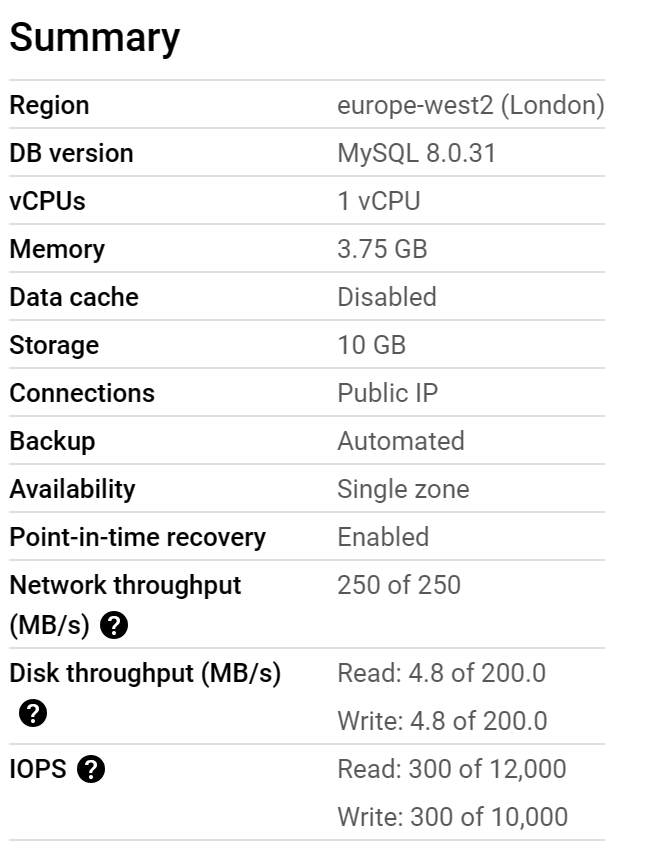
\includegraphics[width=0.5\linewidth]{images/cloud-configurations.png}
    \caption{Google Cloud Configurations}
    \label{fig:cloud-configurations}
\end{figure}

These cloud database costed \$6 to initialise it. The cost per day with these configurations for this database is \$0.4. These configurations are enough for development and testing but when in actual production, these won't work and would create a lag and disrupt the real-time data flow. When in production and used by 100 HCPs and 1 dashboard for 1 hospital, these configurations should change to Enterprise Plus Cloud SQL Edition, with at least 8 vCPU, 32 GB and change storage to at least over 100 GB. This would increase when this platform is used by multiple hospitals. 

In the production, the middleware microservices will also be deployed on Google Cloud. Middleware queries through the database but to do this query, Middleware needs to send a HTTPS request to cloud using unix-socket with all the permissions needed. 

So if admin adds a new device on the dashboard, it goes through Web Page -> Web Server -> Middleware -> Database (on Google Cloud) and the way back. And all this happens using HTTP requests. When Middleware is also deployed on Google Cloud, the transaction between Middleware and Database will reduce, resulting in faster response time. But to do this, would increase the cost of using Google Cloud. And that's why it was not done.


\section{Further Work}
Despite having achieved the core objectives and beyond, there are more enhancements that this project could have done if not for the time constraint and knowledge-specific constraint. Further Work are divided into 3, things to be done to create a minimum viable product, improving current implementations and finally adding new requirements to make VitalMonitor more efficient.

\subsection{Smart Patch: Final Product}
The final device will be made in such a way that it sits behind the ear - where the pulse sensor will be sticked to the ear lobe and the temperature sensor right behind the ear. This prototype can be further made more smaller in size using more efficient chips which are streamlined only for Smart Patch unlike ESP32S3. 

The prototype will be changed from being on the breadboard to a fully soldered device. 

Further research and design will be done to minituarise the device on CAD. 

These can be seen in Figure \ref{fig:fig-design}.

But to even use it on the person a lot of device testing will be involved such as Electrical Safety Testing, Mechanical/Physical Testing. 

This stage didn't do this because it needs much more Electronics knowledge to conduct such testing and due to time constraints I could have not planned it to finish it in this stage. If given more time, I would have delved into this. 

\subsection{Improving the Middleware Infrastructure}
Current Middleware Infrastructure is implemented as one single webserver but in a way that can be easily divided into 4 microservices (on 4 different web servers) and they all collectively will be known as Middleware. These 4 microservices shall be: Session Management Service, User and Device Management Service, Data Ingestion Service and Data Retrieval Service. Isolating these services and have dedicated server to only take care of one thing - this would reduce the burden on one single web server. This along with a load balancer to keep a queue of request to these servers would help streamline the data, making sure no data is lost. This would not only provide separation of concerns and manage requests but would really help in terms of scalability of the system. 

\subsection{Algorithm to Measure Stress and Fatigue Levels}
As discussed in Chapter 2 Literature Review, that there is no defined way of measuring someone's stress or fatigueness in real-time. Because stress and fatigue are so versatile and depends on so many different factors such as physiological and psychological. Further research can be done to use different vitals and personal information to create an algorithm which can measure this in a numerical form rather than just saying ``the person is feeling 'very' stressed". 

Creating this algorithm would involve a lot inputs from medical researches - in order to best evaluate the reasoning and give weights to certain parameters to accurately define a quantitative way to measure stress and fatigue levels. Once this is defined this would just make so much more quicker for decision making. Of course this would involve a lot more data gathering about HCPs but it would reduce the naive approach based on just thresholds on vitals. 

\subsection{Interdisciplinary Collaboration for Enhanced Sensors}
Like previously discussed about the trade off between sensor accuracy and non-intrusiveness. Interdisciplinary collaboration shall be done with electric engineers, bio-medical engineers to develop enhanced sensors which can not only accurately sense the vitals like heart rate and body temperature, SpO2 and salt intensity in sweats but is also non-intrusive to wear. This would pave a path and make a disruption in the healthcare industry. As much as HCPs want it, patients would also like a non-intrusive way of getting medical treatments. This would enhance their overall experience of getting medical treatments - and would make them less suffer in their sufferings already. 


\subsection{Prediction Model}
Stress and Fatigue are not somethings which usually spikes out. Usually there is gradual growth in their levels except for some cases in stress which can spike out when things go sideways out of nowhere or when you hear a very bad news. But usually, one case see the gradual incline or decline. In the future iterations, a prediction model trained of actual human data which can predict before the stress levels go beyond a control line or threshold. This can give warning signals to the admins of the healthcare organization to better prepare for it rather than once the threshold is crossed only then provide the help. This would provide more time to the admin staff to make arrangements. 

Such a model can either be on the middleware predicting in real-time or it can also be on the firmware or a combination of both.  


